\documentclass[../main.tex]{subfiles}

\begin{document}

\problem{5}
Find the output for each of these input strings when given as input to the finite-state machine in Example 2.

\begin{center}
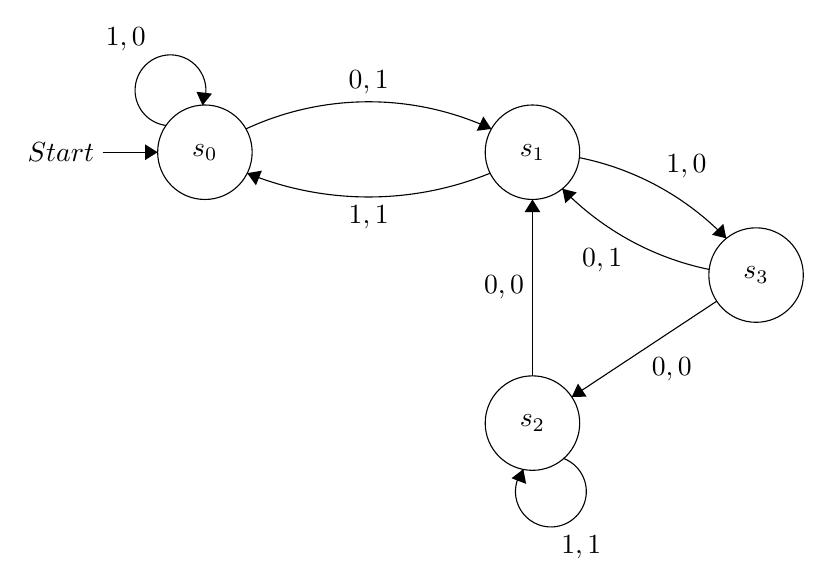
\begin{tikzpicture}[scale=0.2]
\tikzstyle{every node}+=[inner sep=0pt]
\draw [black] (22.1,-21.5) circle (3);
\draw (22.1,-21.5) node {$s_0$};
\draw [black] (42.9,-21.5) circle (3);
\draw (42.9,-21.5) node {$s_1$};
\draw [black] (42.9,-38.7) circle (3);
\draw (42.9,-38.7) node {$s_2$};
\draw [black] (57.1,-29.3) circle (3);
\draw (57.1,-29.3) node {$s_3$};
\draw [black] (15.6,-21.5) -- (19.1,-21.5);
\draw (15.1,-21.5) node [left] {$Start$};
\fill [black] (19.1,-21.5) -- (18.3,-21) -- (18.3,-22);
\draw [black] (24.706,-20.02) arc (114.94743:65.05257:18.479);
\fill [black] (40.29,-20.02) -- (39.78,-19.23) -- (39.36,-20.14);
\draw (32.5,-17.8) node [above] {$0,1$};
\draw [black] (40.214,-22.831) arc (-67.84225:-112.15775:20.454);
\fill [black] (24.79,-22.83) -- (25.34,-23.6) -- (25.72,-22.67);
\draw (32.5,-24.84) node [below] {$1,1$};
\draw [black] (19.643,-19.8) arc (263.0546:-24.9454:2.25);
\draw (17.08,-15.1) node [above] {$1,0$};
\fill [black] (21.95,-18.52) -- (22.55,-17.78) -- (21.56,-17.66);
\draw [black] (54.6,-30.96) -- (45.4,-37.04);
\fill [black] (45.4,-37.04) -- (46.34,-37.02) -- (45.79,-36.19);
\draw (51.75,-34.5) node [below] {$0,0$};
\draw [black] (44.874,-40.944) arc (69.06849:-218.93151:2.25);
\draw (46,-45.83) node [below] {$1,1$};
\fill [black] (42.32,-41.63) -- (41.57,-42.2) -- (42.5,-42.56);
\draw [black] (45.877,-21.844) arc (78.59311:43.84728:17.838);
\fill [black] (55.21,-26.97) -- (55.02,-26.05) -- (54.3,-26.74);
\draw (52.68,-23.19) node [above] {$1,0$};
\draw [black] (54.125,-28.944) arc (-101.60253:-135.95708:18.018);
\fill [black] (44.8,-23.82) -- (44.99,-24.74) -- (45.71,-24.05);
\draw (47.33,-27.59) node [below] {$0,1$};
\draw [black] (42.9,-35.7) -- (42.9,-24.5);
\fill [black] (42.9,-24.5) -- (42.4,-25.3) -- (43.4,-25.3);
\draw (42.4,-30.1) node [left] {$0,0$};
\end{tikzpicture}
\end{center}

\begin{enumerate}[a)]
	\item $0111$
\end{enumerate}


\solution
\begin{enumerate}[a)]
	\item 1100 
\end{enumerate}

\end{document}
